\documentclass[a4paper, 12pt]{scrartcl}
\usepackage{geometry}
\usepackage{setspace}
\geometry{
  textheight = 40\baselineskip,
  outer = 20mm,
  inner = 20mm
}
\usepackage[utf8]{inputenc}
\usepackage{fancyvrb}
\usepackage[italian]{babel}
\usepackage[T1]{fontenc}
\usepackage{graphicx}
\usepackage{underscore}
\usepackage{float}
\usepackage{hyperref}

\graphicspath{ {./} }
\setstretch{1.2}
\setlength{\parindent}{0em}

\begin{document}
    
    \hyphenation{CASCADE}
    
  \section*{Introduzione}
    Gli ultimi anni hanno visto una maturazione dello standard[1 -> link a standard] GraphQL, dei servizi costruiti per implementarlo e la sua adozione da parte di numerose aziende. [2 -> https://graphql.org/users/] \\
    Definito per la prima volta internamente a Facebook nel 2012, oggi si presenta come uno standard capace di competere con l'architettura di tipo REST per il dialogo fra client e server. \\
    Caratterista fondamentale di GraphQL è la possibilità di definire uno schema che permette di modellare il formato delle query esposte e quello delle entità restituite al client, di modo che questo possa effettuare richieste personalizzate, ad un singolo endpoint e vedersi restituire dati già tipizzati. \\
    Le entità sono definite da campi tipizzati e relazioni con altre entità, la struttura del dominio delle interrogazioni gestibili dal server è strutturata come un grafo. \\

    Le possibilità offerte dallo standard però non si limitano alla comunicazione fra client e server: essendo i campi delle entità tipizzati, ed avendo lo standard un concetto di reflection, è possibile usare 
    schemi GraphQL anche per definire lo strato del model. \\
    Questa possibilità rende quindi l'impiego di questo standard potenzialmente adatto per lo sviluppo Model Driven, potendo generare in modo automatizzato il codice applicativo che si occuperà di interfacciarsi con le strutture definite nello schema GraphQL. \\

    Da qualche tempo, l'azienda Twinlogix, ha deciso di sfruttare le potenzialità di questo framework per realizzare un generatore di codice che, basandosi sullo schema, costruisca definizioni di modelli per database. \\
    Per poter interagire con questi modelli, il generatore deve anche generare i \href{https://en.wikipedia.org/wiki/Data_access_object}{DAO} necessari.\\
    A tal scopo, l'azienda sta anche lavorando alla scrittura di un DAO generico e metodi per interagirci indipenti dal tipo dell'oggetto richiesto e dal database sottostante.

    È stato anche scritto un primo prototipo di questo DAO e del generatore per supportare database MongoDB.

    Obiettivi dell'attività di seguito discussa sono stati quindi:
    \begin{itemize}
        \item Studiare le tecnologie necessarie per lo svolgimento dell'attività
        \item Analizzare l'architettura del DAO e i prototipi sviluppati dall'azienda
        \item Progettare e implementare una prima versione versione del DAO generico e del generatore che, sfuttando librerie ORM, potesse interfacciarsi con database SQL.
    \end{itemize}
  \newpage

  \section*{Background}
    \subsection*{Model Driven Programming}
      Lo sviluppo "Model Driven" è un'approccio all'ingegneria del software orientato alla definizione di modelli piuttosto che di software.\\
      Parlare di modelli permette di astrarre la complessità del software, rendendo più chiara la visione dell'interazione fra le varie componenti dell'applicazione.\\
      L'approccio Model Driven è particolarmente efficace quando i suddetti modelli descrivono strutture che si prestano alla generazione automatizzata di codice: così facendo si permette di produrre applicazioni in modo molto più rapido, limitandosi a personalizzare
      i modelli per poi farli generare.\\
      Questo approccio aiuta anche a prevenire l'errore umano: spesso infatti le componenti modellabili e generabili automaticamente presentano strutture complesse, lunghe e difficili da scrivere e gestire personalmente dai programmatori.\\
      Il processo di scrittura, ma anche di aggiornamento, viene quindi privato di errori accidentali, difficili da localizzare, spostando tutta la complessità sui software di generazione del codice.\\
    \newpage

  \section*{Tecnologie}
    \subsection*{GraphQL}
      Ideato da Facebook nel 2012, il linguaggio GraphQL è stato successivamente (nel ?) pubblicato in maniera open source e, dal 2018, è gestito dalla Linux Foundation (moar) come standard.\\
      Nasce con il duplice scopo di modellare entità collegate fra di loro da relazioni e di fornire una soluzione a noti problemi dell'approccio RESTful, architettura per la comunicazione client server prevalente nello sviluppo in ambito web.\\
      Il linguaggio di GraphQL permette di definire uno schema costituito da un punto di ingresso, il nodo root, e uno o più tipi.\\
      
      Questi tipi possono rappresentare: (elenco puntato più espanso) tipi di dato, con i loro rispettivi campi, "richieste", "mutazioni", enum etc\dots\\
      
      Ogni tipo al suo interno piò contenere uno o più scalari, ovvero valori foglie, e uno o più altri oggetti complessi: in questo modo vengono definite le relazioni fra le varie entità.\\

      Quando un client contatta un server GraphQL, può fornire come parametri di richiesta operazioni di query o mutazione definita nello schema definenendo, specificandone i vari campi, quale forma avrà il risultato restituito dall'operazione.\\

      Le immagini successive mostrano un esempio di comunicazione con un server GraphQL in contrasto ad uno con uno utilizzante l'API REST
      https://www.howtographql.com/basics/1-graphql-is-the-better-rest/\\


      Si nota quindi che l'utilizzo di GraphQL permette di risolvere due grandi problemi dell'approccio REST:
      \begin{itemize}
        \item 
        Overfetching underfetching "This happens because the only way for a client to download data is by hitting endpoints that return fixed data structures"
        \item
        Inoltre, essendo specificato solo un punto d'ingresso nello schema (il nodo root), questo diventa anche l'unico endpoint che un clint dovrà contattare, evitando di dover inviare più richieste per accedere a dati associati. 
      \end{itemize}
      
      Necessità di modifcare backend in caso di cambiamenti a frontend -> da espandere \\
      Il fatto che lo schema indichi campi tipizzati rende pure molto più semplice la comprensione delle risposte da parte del server. -> spiega \\

      Essendo uno standard, GraphQL non è legato ad implementazioni o tecnologie. Lavorando in ambito NodeJS, in questo elaborato verrrà utilizzato Apollo Server[link].

      GraphQL comprende il concetto di reflection! (espandi)

      GraphQL può essere usato come linguaggio per definire modelli: sono infatti già disponibili servizi di generazione di codice basata su schemi GraphQL.\\
      Quello utilizzato in questo caso è "GraphQL-code-generator" [link].

    \subsection*{Graphql code generator}
      GraphQL code generator è un tool CLI open source, rilasciato nel XXXX da YYYY, in grado di analizzare uno schema GraphQL e, tramite plugins, generare codice.\\
      Il modo in cui questo strumento opera è utilizzando il pattern di programmazione "visitor".
      \subsubsection*{Pattern Visitor}
        Il pattern visitor è una soluzione al problema che si verifica quando bisogna effettuare operazioni su una struttura di oggetti senza però aggiungere funzionalità agli stessi:\\
        ogni oggetto della struttura implementa un'interfaccia che definisce un metodo "accept" che riceve come parametro un'implementazione dell'interfaccia Visitor.\\
        L'interfaccia Visitor specifica invece un metodo "visit" per ogni tipologia (ad esempio, ogni classe) di oggetto sul quale svolgere operazioni.\\
        Nell'applicazione principale poi, per ogni oggetto, viene chiamato il metodo accept passando ogni implementazione di Visitor, cosicchè per aggiungere operazioni/trasformazioni delle classi è possibile semplicemente implementare un nuovo Visitor.\\

        È questo il meccanismo alla base di GraphQL code generator: al suo interno, ogni plugin può accedere allo schema del grafo e chiamare il metodo \emph{visit}, passando come parametro un oggetto che funga da visitor.

        Sono disponibili dei plugin predefiniti, fra cui quello, usato durante questo progetto, per generare tipi, interfacce etc... in linguaggio TypeScript.

    \subsection*{TypeScript}
      [parla dei tipi avanzati]

    \subsection*{Sequelize}
      Di accordo con l'azienda, la versione SQL è stata scritta sfruttando la libreria ORM "Sequelize" per l'interazione con la base di dati. (Perchè Sequelize e non typeORM?)

      \subsubsection*{ORM}
        L'Object Relational Mapping è una tecnica di programmazione creata per favorire l'interazione fra un'applicazione scritta con un approccio ad oggetti ed una base di dati di tipo relazionale, o comunque modellante tabelli tramite campi scalari semplici.\\
        Una libreria ORM, infatti, rende possibile mappare le tabelle a degli oggetti e viceversa, permettendo pertanto di poter operare con questi dentro l'applicazione anche quando si deve comunicare con un DB.\\

        [Esempi?
            -inserimento oggetti in un DB\\
            -fetch oggetti da un DB
        ]

        Gli immediati vantaggi di questo approccio sono il ridotto numero di linee di codice scritte, nonchè la semplicità nell'interazione con il DB.\\
        Un altro importante vantaggio, prendendo ad esempio il caso di Sequelize, è il fatto di poter astrarre più facilmente anche l'implementazione del DataBase utilizzato e rendere più veloce la connesione con questo.\\

        [
            Esempi di connessione\\
            Esempio di query tradotta in modo diverso fra un db e l'altro
        ]

        D'altro canto, utilizzare una libreria ORM ha anche numerosi svantaggi:
        \begin{itemize}
          \item E' una libreria complessa se la si vuole sfruttare a fondo
          \item Bisogna effettuare un setup
          \item Toglie del controllo al programmatore vista la grande astrazione che introduce
          \item Può produrre query subottimali
        \end{itemize}
        Questi svantaggi non sono però stati ritenuti abbastanza influenti da decidere di optare per una soluzione di più basso livello.\\
  \newpage
  \section*{Requisiti}
    TODO

  \newpage
  \section*{Testing}
    TODO

  \newpage  
  \section*{Architettura del prototipo}
    L'interazione con lo strato del database è gestita tramite il pattern di programmazione Data Access Object (DAO).\\
    Il pattern DAO è una strategia impiegata per separare lo strato funzionale di un'applicazione da quello di persistenza dei dati: permette quindi di sviluppare il lato applicativo senza avere conoscenza di come i dati vengano effettivamente gestiti, così come poter modificare la gestione dei dati
    senza dover effettuare modifiche al lato applicativo, a patto che le interfacce rimangano inalterate.\\
    Il pattern prevede la definizione di un'interfaccia di alto livello che definisce i metodi di lettura e scrittura su un particolare tipo di oggetto, l'implementazione di questa e dell'oggetto, detto "Data Transfer Object", che non è altro che un'entità sulla quale mappare i dati custoditi nel DataBase.\\
    
    \begin{figure}[H]
      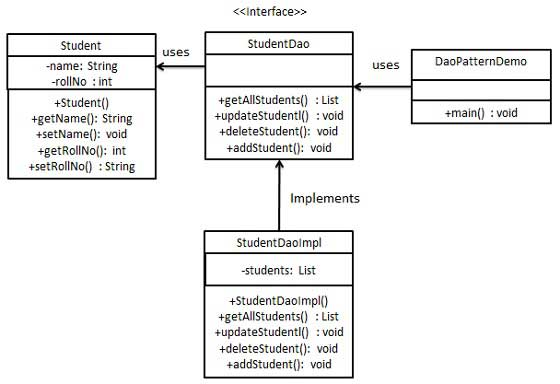
\includegraphics[width=\textwidth]{dao_pattern_uml_diagram.jpg}
      \caption{Esempio di pattern DAO. Fonte: \href{https://www.tutorialspoint.com/design_pattern/images/dao_pattern_uml_diagram.jpg}{www.tutorialspoint.com}}
    \end{figure}

    Dovendo però scrivere dei dao per oggetti che verranno generati in futuro, l'implementazione aziendale del pattern punta a definire un generico DAO adatto a qualsiasi tipo di DTO, con metodi quindi non personalizzati in base ad esso.\\
    La struttura della libreria è quindi composta da una interfaccia che definisce un dao di lettura ed una che definisce operazioni di un generico dao, estendente quella del dao di lettura.
    Queste operazioni (find, count, insert, delete...) prendono come parametri filtri, proiezioni, ordinamenti etc... che verranno poi generati dal generatore in base al tipo del DTO.\\

    Viene anche definito un meccanismo di associazioni tra dao indipendente dal database sottostante, così da poter implementare associazioni fra i vari tipi dello schema graphql anche in database privi del concetto di associazione.\\

    Infine, è definito un DAO astratto che implementa le operazioni descritte nelle interfacce tramite metodi template.\\
    La comunicazione con lo strato di persistenza è delegata a implementazioni della classe DAO astratta.\\
  \newpage
  \section*{Sviluppo del DAO}
    \subsection*{Individuazione delle problematiche}
      Le problematiche maggiori della fase di implemetazione del DAO astratto sono scaturite dalle differenze fra database di tipo documentale (come MongoDB) e database SQL.\\
      Gli schemi GraphQL utilizzati dall'azienda per eseguire test, e che sono stati presi come punto di riferimento per lo sviluppo dell'implementazione, presentano alcuni tipi difficilmente convertibili in maniera triviale, questo perchè gli schemi GraphQL sono
      particolarmente adatti per definire modelli che si adattano bene a documenti.

      I database documentali non sono basati su tabelle rigidamente definite, ma contengono al loro interno documenti, oggetti codificati in diversi standard (XML, JSON, YAML...), non strutturati e conservati in una singola istanza, piuttosto che essere potenzialmente distribuiti in più tabelle.
      
      [immagini con esempi di entrambi i db e didascalie]

      Di seguito è mostrato un esempio di tipo dalla difficile mappatura in un database SQL:
      \begin{Verbatim}[samepage=true]
        type Person implements Account {
            id: ID!
            name: String!
            address: Address
            dog: Dog
            amount: Float
            dogSittersId: [ID!]
            dogSitters: [DogSitter!] @mongoInnerRef
            beagleId: ID!
            beagle: Beagle @mongoInnerRef
        }
      \end{Verbatim}

      I campi seguiti dalla direttiva \emph{@mongoInnerRef} non sono mappati sul database, ma verranno gestiti come associazioni con il meccanismo di associazioni fra dao.\\
      I problemi di tipi come questo sono dunque:
      \begin{itemize}
        \item Il tipo estende un'interfaccia
        \item Al suo interno il tipo contiene un campo di un altro tipo: \emph{Address} (questi tipi non rappresentano tabelle sulle quali effettuare richieste direttamente, ma sono tipi innestati nei tipi delle tabelle)
        \item Al suo interno il tipo contiene un campo di tipo interfaccia: \emph{Dog}
        \item Al suo interno il tipo contiene degli array
      \end{itemize}

      Questi problemi, non sono esistenti se alla base è usato un database documentale: i documenti possono infatti possedere campi di tipi composti e array nativamente.\\

      Anche l'interazione con i dao che gestiscono tipi complessi come quello appena segnalato presenta problematiche: è infatti previsto, almeno nella versione mongoose, che si possa interagire con i dao delle interfacce come se si stessero interrogando anche i dao delle implementazioni.
      Per esempio, dati i tipi
      \begin{Verbatim}[samepage=true]
        interface User @mongoEntity {
          id: ID! @id
        }

        type ProfessionalUser implements User {
          id: ID!
          profile: ProfessionalProfile
        }
      \end{Verbatim}

      mappati in tipi TypeScript nel seguente modo

      \begin{Verbatim}[samepage=true]
        export type User = {
          id: Scalars['ID'];
        };
        export type ProfessionalUser = User & {
          __typename?: 'ProfessionalUser';
          id: Scalars['ID'];
          profile?: Maybe<ProfessionalProfile>;
        };
      \end{Verbatim}

      dovrebbe essere possibile effettuare la seguente operazione

      \begin{Verbatim}[samepage=true]
        let user : (User | null) = 
          await dao.user.insert({ firstName: "FirstName", live: true });
        let customerUser : CustomerUser = 
          { id: user.id, __typename: "CustomerUser",
            firstName: "FirstName 1", organizationId: "organization_id",
            live: true };
        await dao.user.replace(user, customerUser);
      \end{Verbatim}

      ed aspettarsi, interrogando successivamente il dao di user, di ricevere in risposta il record di tipo CustomerUser.

    \newpage
    \subsection*{Risoluzione delle problematiche - alto livello}
      In un primo momento era stato ipotizzato di gestire i casi sopra descritti con delle associazioni, sfruttando il meccanismo di riferimenti già presente nel progetto dell'azienda.\\
      Questo approccio avrebbe però portato a dover gestire una serie di complicazioni:
      \begin{itemize}
        \item Generazione manuale delle tabelle fittizie per gestire gli array di primitive
        \item Necessità di dover creare un meccanismo di gestione delle interfacce non banale
        \item Gestire manualmente aggiornamento, eliminazione, sostituzione etc... di un entità con altri tipi innestati
        \item Generazione manuale delle tabelle di giunzione per gestire le relazioni fra tipi
        \item Necessità di effettuare modifiche all'interfaccia delle associazioni, quindi dover modificare l'interfaccia del dao comune
        \item Dipendenza di associazioni l'una dall'altra: è per esempio possibile che un'associazione interna dipenda da un campo contenuto in un oggetto innestato; essendo, nel caso SQL, l'oggetto embedded rappresentato da un'altra associazione, sarebbe stato necessario definire un meccanismo per rilevare e gestire le dipendenze fra queste.
      \end{itemize}
      
      Pertanto, sono stati invece evitati alcuni fra questi problemi (in particolare gli ultimi tre) usando le associazioni di Sequelize.\\
      (nota: verrà usato il termine \emph{riferimenti} per riferirsi alle associazioni indicate su schema GraphQL e risolte tramite il meccanismo interno al DAO, mentre \emph{associazioni} per intendere associazioni Sequelize)\\
      Non usando il meccanismo di gestione dei riferimenti si evita di dover effettuare cambiamenti all'interfaccia comune e non bisogna gestire dipendenze fra essi, in quanto la loro risoluzione verrà eseguita solo dopo che il dao Sequelize avrà raccolto tutti i dati della tabella e di quelle associate.\\
      Oltre a questo, Sequelize gestisce in autonomia (o dietro configurazione esplicita) la creazione di foreign keys per collegare le tabelle fra di loro, non rendendo necessario aggiungere questi campi, utili solo alla versione SQL, nello schema GraphQL.\\

      I campi di tipi embeddedd verranno mappati in tabelle secondarie, con riferimenti alle tabelle alle quali appartengono.\\
      Gli array vengono gestiti tramite l'associazione Sequelize di tipo HasMany: nel caso siano array di dati scalari, verrà creata una tabella apposita per contenere questi valori. \\
      Per la gestione delle interfacce è stato scelto di tenere tutti i campi comuni in una tabella relativa all'interfaccia, mentre in quelle delle implementazioni saranno salvati i dati relativi ad esse ed un riferimento al record associato sulla/e tabella/e dell'interfaccia/e.
      Viene aggiunto, dove non indicato nello schema graphql, un campo id fittizio.

      Per gestire le tabelle aggiuntive verranno inizializzati dei dao dedicati, tenendoli però nascosti all'utilizzatore dell'applicazione.

      Il tipo precedentemente mostrato e quelli associati verranno quindi mappati con la seguente struttura di tabelle\\
      
      \begin{figure}[H]
        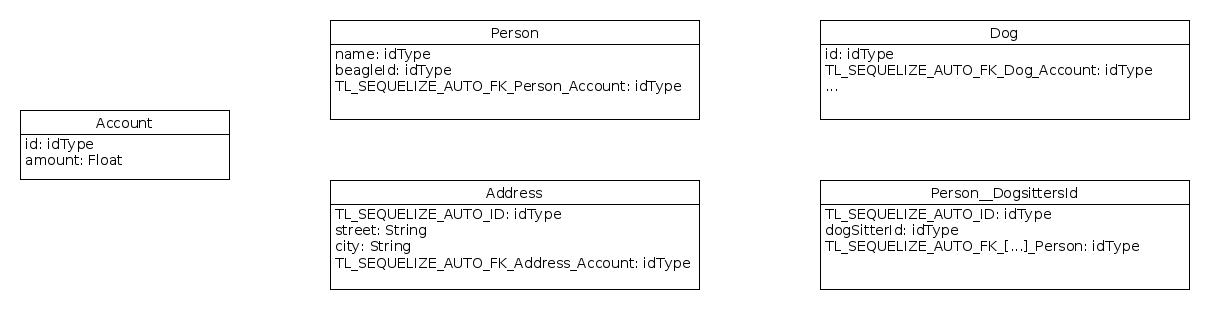
\includegraphics[width=\textwidth]{db-example.png}
        \caption{I campi aggiuntivi sono quelli con la dicitura \emph{TL_SEQUELIZE_AUTO}.\\Person_dogSittersId è una tabella aggiunta, che serve per contenere i valori dell'array \emph{dogSittersId}}
      \end{figure}

      Per gestire le associazioni fra dao è stata definita la seguente interfaccia:
      \begin{Verbatim}[samepage=true]
        interface SequelizeAssociation {
          field : string,
          daoModelName : string,
          kind : SequelizeAssociationKind
          alias: string,
          extractField? : string,
        }
      \end{Verbatim}
      Ogni dao conserva una mappa che, al nome di un campo, associa una tupla composta dal dao associato a quel campo e dalla SequelizeAssociation corrispondente.
      Il significato dei campi è il seguente:
      \begin{itemize}
        \item field: nome del campo associato ad un altro dao
        \item daoModelName: nome del dao associato
        \item kind: indica se il dao associato rappresenta un tipo \emph{embedded}, \emph{interfaccia} o \emph{implementazione}
        \item alias: alias dell'associazione SQL fra i modelli dei dao
        \item extractField: opzionale. Se utilizzato in un'associazione di tipo embedded, indica che il/i model associati dovranno essere mappati al campo indicato.
                            Nell'applicazione, verrà usato per gestire gli array di primitive.
      \end{itemize}
      Il principio di funzionamento generale dell'apllicazione è quindi quello di rilevare quando un campo presente nei parametri della query è relativo ad un dao associato e, di conseguenza, delegare la risoluzione di quel campo al dao.
    \newpage

    \subsection*{Risoluzione delle problematiche - implementazione}
      Le funzioni principali del dao astratto da implementare sono:
      \begin{itemize}
        \item Insert - Inserimento.
        \item Find   - Ricerca
        \item Update - Aggiornamento
        \item Delete - Eliminazione
      \end{itemize}
      Tutte le altre operazioni (come \emph{count} e \emph{replace}) sono derivabili da queste.\\

      Per gestire le associazioni, molti dei metodi scritti hanno una struttura ricorsiva del tipo:
      \begin{Verbatim}[samepage=true]
        function recursiveFunction(query, ...) {
          for(let field in query) {
            const a = this.sequelizeAssociations.get(field)
            if (a) {
              if(a is of kind EMBEDDED) {
                a.getDao().recursiveFunction(query[field])
              } else {
                a.getDao().recursiveFunction({field : query[field]})
              }
            }
            ...
          }
        }
      \end{Verbatim}
      Se un'associazione viene rilevata su un campo del parametro query, la funzione verrà richiamata sul dao associato a quel campo. 
      Bisogna però fare attenzione al tipo di associazione: se è di tipo embedded, il dao associato si occuperà di gestire direttamente il dato passato. Altrimenti, vuol dire che il dao associato è una interfaccia o implementazione e potrebbe dover
      delegare nuovamente il campo ad un dao associato in modo embedded.

    \newpage
    \subsection*{Inserimento}
      [signature?]
      Per l'inserimento è definita una sola funzione, che accetta il record da inserire nel database ed eventuali opzioni di scrittura.
      Sequelize permette di effettuare l'operazione di inserimento passando direttamente un oggetto composto, a patto di includere le associazioni alle tabelle relative
      nel parametro "options" di input.
      \begin{Verbatim}[samepage=true]
        return Product.create({
            title: 'Chair',
            user: {
                firstName: 'Mick',
                addresses: [{
                    city: 'Austin',
                },{
                    city: 'New York',
                }]
            }
            }, {
            include: [{
                association: Product.User,
                include: [ User.Addresses ]
            }]
        });
      \end{Verbatim}
      Esempio di inserimento di un oggetto di tipo Product, uno User associato e indirizzi associati allo user.

      L'inserimento pertanto viene eseguito in due fasi:\\
      Nella prima, il record passato in input viene processato e tutti i suoi campi associati vengono raggruppati dietro all'\emph{alias} delle associazioni.\\
      Nel caso dell'esempio precedente, in un oggetto di tipo
      \begin{Verbatim}[samepage=true]
        {
          title: 'Chair', 
          firstName: 'Mick',
          addresses: [{city: 'Austin}, ...]
        }
      \end{Verbatim}
      passato come input al dao "product", vengono rilevate le associazioni ai campi "firstName" e "addresses" e raggruppate dietro l'alias ("user") dell'associazione, come mostrato nell'esempio sopra.
      Ricorsivamente, nel dao "user", viene gestito il campo associato "addresses".\\

      Nella seconda fase viene invece costruito l'oggetto delle opzioni che deve ricorsivamente indicare tutte le associazione incluse nella query.

    \newpage
    \subsection*{Ricerca}
      \subsubsection*{Interfaccia di Sequelize}
        Sequelize permette di effettuare un'operazione di ricerca includendo subito uno o più modelli associati, tramite il meccanismo di Eager Loading.

        Esempio di semplice query di ricerca con un modello associato, nella quale viene indicato anche l'alias dell'associazione:
        \begin{Verbatim}[samepage=true]
          const users = await User.findAll({
            include: { model: Tool, as: 'Instruments' }
          });
        \end{Verbatim}
        
        È possibile, in alternativa al passare la coppia di attributi "model"/"as", definire un campo "association", inizializzato con il nome dell'associazione.
        \begin{Verbatim}[samepage=true]
          User.findAll({ include: { association: 'Instruments' } });
        \end{Verbatim}

        È anche supportata l'inclusione di più modelli alla volta, nonchè di modelli associati a quelli inclusi, in modo innestato.
        \begin{Verbatim}[samepage=true]
          User.findAll({ include: [
                                    { association: 'Instruments' }, 
                                    { association: 'Tools', 
                                      include : [
                                        association : 'Designers'
                                      ]
                                    }
                                  ]});
        \end{Verbatim}

        Tramite l'opzione \emph{where} è invece possibile definire un filtro per la ricerca.
        \begin{Verbatim}[samepage=true]
          User.findAll({
            where : {firstName : 'Paul'},
            include: {
              association: 'Instruments',
              where: {
                size: {
                  [Op.ne]: 'small'
                }
              }
            }
          });
        \end{Verbatim}

        Definire così le opzioni di ricerca scollegerebbe i filtri dei campi di una tabella da quelli dei campi di una tabella che rappresenterebbe un'oggetto innestato in quella precedente.
        Ad esempio, supponendo che l'associazione "Instruments" rappresenti un oggetto embedded in User, il filtro di ricerca
        \begin{Verbatim}[samepage=true]
          userFilter : UserFilter = {
            $or : {
              firstName : 'Paul', 
              "Instruments.size" : {
                $ne : 'small'
              }
          }}
        \end{Verbatim}
        Non sarebbe traducibile, non potendo mettere in "OR" i due filtri, secondo la modalità precendente presentata.
          
        Fortunatamente, Sequelize permette di elevare allo stesso livello tutti i filtri, risolvendo così il problema.
        \begin{Verbatim}[samepage=true]
          User.findAll({
            where : {
              [Op.or] : {
                "$firstName$" : 'Paul', 
                "$Instruments.size$" : {
                  [Op.ne] : 'small'
                }
              }
            },
            include: {
              model: Tool,
              as: 'Instruments'
            }
          });
        \end{Verbatim}

        È possbile indicare, per ogni modello incluso, una lista di attributi da estrarre. Grazie a questo è possibile implementare la proiezione di attributi.

        L'ordinamento, similmente ai filtri, è specificabile sia modello per modello che al livello radice della query. Quest'ultima opzione è stata scelta.

        Ad esempio, l'ordinamento
        \begin{Verbatim}[samepage=true]
          userSort : UserSort = [
            {firstName : SortDirection.ASC},
            {"Instruments.size" : SortDirection.DESC}
          ]
        \end{Verbatim}
        può esere tradotto in una query Sequelize nel seguente modo:
        \begin{Verbatim}[samepage=true]
          User.findAll(
            {
              order: [
                ['firstName', 'ASC'],
                ['Instruments', 'size', 'DESC']
              ]
              include: {
                model: Tool,
                as: 'Instruments'
              }
            });
        \end{Verbatim}

      \subsubsection*{Implementazione}
        Sequelize permetterebbe di effettuare automaticamente un join fra il Model iniziale, tutti quelli associati e potenzialmente anche quelli associati a quelli assocciati tramite l'opzione, da inserire nella query,
        \emph{attributes: \{all : true, nested : true\}}.\\
        Questo semplificherebbe di molto il problema della gestione della query, ma ogni interrogazione comporterebbe un numero elevato di operazioni di join.\\
        Per ridurre il numero di join dunque l'implementazione della ricerca cercherà di includere solo le tabelle strettamente necessarie.\\

        A tal proposito, vengono analizzati filtri, proiezioni e ordinamenti ricevuti in input per identificare i modelli da includere nella ricera.

        Per fare ciò, i parametri in input vengono tradotti, dove serve, sia in un fomato comprensibile per Sequelize, sia in un oggetto a più livelli per facilitare l'individuazione di campi associati.\\

        Per esempio, il filtro "userFilter" precedentemente mostrato viene convertito in
        \begin{Verbatim}[samepage=true]
          {
            $or : {
              firstName : 'Paul',
              Instruments : {
                size : {
                  $ne : 'small'
                }
              }
            }
          }
        \end{Verbatim}

        così da poter, rilevare, percorrendo ricorsivamente la struttura, l'associazione con il model Tool sul campo Instruments.
        [Schema del processo di ricerca?]

    \newpage
    \subsection*{Aggiornamento}
      Sono rese disponibili tre funzioni di aggiornamento: 
      \begin{itemize}
        \item update: accetta un oggetto di tipo ModelType, lo cerca di individuare nel database ed aggiornarlo
        \item updateOne: accetta un filtro di ModelType e aggiorna il primo record individuato in base ad esso
        \item updateMany: accetta un filtro di ModelType e aggiorna tutti i record individuati in base ad esso
      \end{itemize} 
      Tutte e tre le funzioni ricevono anche in input un oggetto per definire gli aggiornamenti da scrivere.

      L'operazione di aggiornamento con modelli associati non è correntemente supportata da Sequelize, quindi è stato implementato il seguente procedimento:\\
      \begin{enumerate}
        \item Viene eseguita un'operazione di ricerca per ottenere tutti i modelli da modificare in base al filtro passato alla funzione
        \item Per ogni campo dell'oggetto che indica i cambiamenti, si controlla se il nome di questo campo corrisponde a quello di un'associazione
        \item In caso positivo, per ogni modello da aggiornare, bisogna verificare se il campo di quel modello è un array
        \begin{itemize}
          \item Nel caso lo sia, l'array va sostituito completamente con quello passato in ingresso. Vengono quindi cancellati tutti i modelli associati con il modello preso in esame e
          successivamente inseriti e associati nuovi modelli sulla base dei cambiamenti passati.
          \item Altrimenti, se il campo non è vuoto, la funzione di aggiornamento viene richiamata ricorsivamente passando come parametri i cambiamenti sul campo corrente e il modello da aggiornare (sempre facendo caso al tipo di associazione rilevata)
        \end{itemize}
        \item Alla fine, vengono mappati tutti i modelli da aggiornare ai loro id, per poter eseguire un'unica operazione di aggiornamento in blocco sulla tabella sfruttando come filtro la lista di id, piuttosto che chiamare la funzione di aggiornamento per ogni modello (effettuando quindi n operazioni di update).
      \end{enumerate}
        
      [flowchart?]

    \newpage
    \subsection*{Eliminazione}
      Le funzioni di eliminazione da implementare sono due:
      \begin{itemize}
        \item deleteOne: funzione che riceve in input un oggetto e cerca di eliminare il record equivalente nel database
        \item deeteMany: funzione che riceve in input un filtro e cerca di eliminare tutti i record del database che lo soddisfano
      \end{itemize}

      L'eliminazione di un modello e di tutte le sue associazioni di tipo hasOne/hasMany è gestita automaticamente da Sequelize impostando nell'associazione l'opzione sql ONDELETE CASCADE.
      Questo però non copre l'eliminazione delle interfacce associate (belongsTo) nel caso si chiami l'operazione \emph{delete} sul dao di una implementazione: per gestirle vengono raccolte tutte le sequelizeAssociations di tipo "interfaccia" e si chiama l'operazione di eliminazione sui dao associati.\\

      L'implementazione dei modelli Sequelize della funzione di delete accetta fra i parametri un filtro per indicare quali record andranno eliminati, ma non permette però di includere nel filtro campi di altre tabelle (come nel caso della ricerca).
      Nel caso dell'operazione deleteMany quindi, sarà prima necessario recuperare tutti i models da eliminare con una ricerca per poi mapparli sui loro id, così da rendere il filtro per l'operazione di delete corretto, lo stesso procedimento viene effettuato anche sulle interfacce.

    \newpage
    \section*{Sviluppo del generatore}
      Il sistema per la generazione dei modelli è stato suddiviso, seguendo la struttura già adottata dall'azienda, nei seguenti moduli:

      \begin{itemize}
        \item Un plugin per graphql-code-generator per tenere in comunicazione gli altri moduli
        \item Un file per gestire il trattamento dei nodi del modello GraphQL (implementando il pattern visitor)
        \item Un generatore per verificare la validità dei nodi e invocare metodi di generazione
        \item Un generatore astratto per contere metodi comuni e le sue implementazioni:
        \begin{itemize}
          \item Un generatore per generare gli schemi Sequelize
          \item Un generatore per generare dao e tipi di supporto
        \end{itemize}
      \end{itemize}

      [Schema dell'esecuzione]

      \paragraph*{Modulo visitor}
      Viene definito un oggetto che estende la classe \emph{BaseVisitor} di graphql-codegen ed implementa metodi \emph{visit} per gestire definizioni di tipi ed interfacce.

      Nodi interfaccia e tipo vengono trattati in modo quasi identico e il loro trattamento genera uno o più oggetti (nel caso sia necessario creare tabelle di supporto per quella principale) di tipo \emph{TsSequelizeGeneratorNode}.
      \begin{Verbatim}[samepage=true]
        export enum NodeTypes {
          INTERFACE,
          TYPE,
          EMBEDDED
        }

        export type TsSequelizeGeneratorNode = {
          type?: NodeTypes
          name: string
          isAutoGenerated: boolean
          collection: string
          interfaces: string[]
          fields: TsSequelizeGeneratorField[]
          ...
        }       
      \end{Verbatim}
      Campi principali del tipo TsSequelizeGeneratorNode:
      \begin{itemize}
        \item type: è assente se il nodo è autogenerato (vedere in seguito), altrimente prende uno dei valori dell'enum NodeTypes.
        \item name: nome del nodo
        \item isAutoGenerated: identifica se il nodo è stato aggiunto pur non essendo presente nello schema GraphQL. In particolare, identifica i nodi creati per gestire array di dati primitivi.
        \item collection: nome della tabella nel database
        \item interfaces: nome delle interfacce del nodo
        \item fields: collezione contenente i campi del nodo trattato
      \end{itemize}
      \newpage

      \paragraph*{Modulo generatore}
      Il modulo di generazione, invocato dal plugin dopo aver raccolto tutti i nodi trattati, analizza ognuno di questi e ne controlla la correttezza.\\
      In particolare, viene verificato che:
      \begin{itemize}
        \item Ogni nodo abbia un campo id o almeno una interfaccia con un campo tale.
        \item I campi sui quali i riferimenti (segnalati tramite direttiva @sqlizeForeignRef o @sqlizeInnerRef) si basano siano esistenti.
        \item I campi condivisi fra implemetazioni ed interfacce siano di tipo compatibile.
      \end{itemize}

      Dentro la classe del generatore è contenuta una lista di implementazioni di generatore del file finale, tutti implementanti una classe astratta.\\
      Dopo aver controllato tutti i punti precedenti, il generatore principale invoca i metodi di generazione di imports, definizioni ed exports dei generatori della lista.

      \paragraph*{Generatore degli schemi db}
      Il generatore degli schemi di Sequelize analizza tutti i nodi, generando per ciascuno un model Sequelize.
      Gli attributi del model generato corrispondono ai campi del nodo che:
      \begin{itemize}
        \item Non hanno direttive di tipo "reference" nello schema
        \item Non appartengono ad interfacce
        \item Non sono etichettati come liste
        \item Non sono etichettati come di tipo embedded
      \end{itemize}

      \paragraph*{Generatore dei dao}
      Per ogni nodo generato dal visitor, il generatore dei dao verifica in primo luogo se l'attributo "isAutoGenerated" è impostato.\\
      Nel caso lo sia, significa che il nodo non è parte dello schema GraphQL e che quindi il plugin di generazione dei tipi typescript, lanciato prima del plugin personalizzato descritto in queste sezioni, non ha generato un tipo relativo ad esso.\\
      Il generatore dei dao deve quindi definire tipi per gestire i nodi autogenerati poichè gli oggetti di tipo SequelizeAbstractDAO richiedono fra i parametri generici anche il tipo del DTO.

      Il generatore dei dao si occupa anche, per ogni nodo, di generare filtri, proiezioni e ordinamenti sulla base dei campi del nodo.

      Infine, per ogni nodo, genera l'oggetto di tipo dao, inizializzandolo con i corretti riferimenti e sequelizeAssociations.

    \newpage
    \section*{Limiti dell'implementazione proposta}

    \newpage
    \section*{Conclusioni}

    \newpage
    \section*{Bibliografia}
          \href{https://hostname.com}{placeholder} \\
\end{document}